\PassOptionsToPackage{unicode=true}{hyperref} % options for packages loaded elsewhere
\PassOptionsToPackage{hyphens}{url}
\PassOptionsToPackage{dvipsnames,svgnames*,x11names*}{xcolor}
%
\documentclass[8pt,ignorenonframetext,dvipsnames]{beamer}
\usepackage{pgfpages}
\setbeamertemplate{caption}[numbered]
\setbeamertemplate{caption label separator}{: }
\setbeamercolor{caption name}{fg=normal text.fg}
\beamertemplatenavigationsymbolsempty
% Prevent slide breaks in the middle of a paragraph:
\widowpenalties 1 10000
\raggedbottom
\setbeamertemplate{part page}{
\centering
\begin{beamercolorbox}[sep=16pt,center]{part title}
  \usebeamerfont{part title}\insertpart\par
\end{beamercolorbox}
}
\setbeamertemplate{section page}{
\centering
\begin{beamercolorbox}[sep=12pt,center]{part title}
  \usebeamerfont{section title}\insertsection\par
\end{beamercolorbox}
}
\setbeamertemplate{subsection page}{
\centering
\begin{beamercolorbox}[sep=8pt,center]{part title}
  \usebeamerfont{subsection title}\insertsubsection\par
\end{beamercolorbox}
}
\AtBeginPart{
  \frame{\partpage}
}
\AtBeginSection{
  \ifbibliography
  \else
    \frame{\sectionpage}
  \fi
}
\AtBeginSubsection{
  \frame{\subsectionpage}
}
\usepackage{lmodern}
\usepackage{amssymb,amsmath}
\usepackage{ifxetex,ifluatex}
\usepackage{fixltx2e} % provides \textsubscript
\ifnum 0\ifxetex 1\fi\ifluatex 1\fi=0 % if pdftex
  \usepackage[T1]{fontenc}
  \usepackage[utf8]{inputenc}
  \usepackage{textcomp} % provides euro and other symbols
\else % if luatex or xelatex
  \usepackage{unicode-math}
  \defaultfontfeatures{Ligatures=TeX,Scale=MatchLowercase}
\fi
% use upquote if available, for straight quotes in verbatim environments
\IfFileExists{upquote.sty}{\usepackage{upquote}}{}
% use microtype if available
\IfFileExists{microtype.sty}{%
\usepackage[]{microtype}
\UseMicrotypeSet[protrusion]{basicmath} % disable protrusion for tt fonts
}{}
\IfFileExists{parskip.sty}{%
\usepackage{parskip}
}{% else
\setlength{\parindent}{0pt}
\setlength{\parskip}{6pt plus 2pt minus 1pt}
}
\usepackage{xcolor}
\usepackage{hyperref}
\hypersetup{
            pdftitle={Introduction to Multivariate Regression \& Program Evaluation},
            pdfauthor={Lecture 14},
            colorlinks=true,
            linkcolor=Maroon,
            filecolor=Maroon,
            citecolor=Blue,
            urlcolor=blue,
            breaklinks=true}
\urlstyle{same}  % don't use monospace font for urls
\newif\ifbibliography
\usepackage{graphicx,grffile}
\makeatletter
\def\maxwidth{\ifdim\Gin@nat@width>\linewidth\linewidth\else\Gin@nat@width\fi}
\def\maxheight{\ifdim\Gin@nat@height>\textheight\textheight\else\Gin@nat@height\fi}
\makeatother
% Scale images if necessary, so that they will not overflow the page
% margins by default, and it is still possible to overwrite the defaults
% using explicit options in \includegraphics[width, height, ...]{}
\setkeys{Gin}{width=\maxwidth,height=\maxheight,keepaspectratio}
\setlength{\emergencystretch}{3em}  % prevent overfull lines
\providecommand{\tightlist}{%
  \setlength{\itemsep}{0pt}\setlength{\parskip}{0pt}}
\setcounter{secnumdepth}{0}

% set default figure placement to htbp
\makeatletter
\def\fps@figure{htbp}
\makeatother


%packages
\usepackage{graphicx}
\usepackage{rotating}
\usepackage{hyperref}

\usepackage{tikz} % used for text highlighting, amongst others
\usepackage{comment}

%title slide stuff
%\institute{Department of Education}
%\title{Managing and Manipulating Data Using R}

%
\setbeamertemplate{navigation symbols}{} % get rid of navigation icons:
\setbeamertemplate{footline}[page number]

%\setbeamertemplate{frametitle}{\thesection \hspace{0.2cm} \insertframetitle}
\setbeamertemplate{section in toc}[sections numbered]
%\setbeamertemplate{subsection in toc}[subsections numbered]
\setbeamertemplate{subsection in toc}{%
  \leavevmode\leftskip=3.2em\color{gray}\rlap{\hskip-2em\inserttocsectionnumber.\inserttocsubsectionnumber}\inserttocsubsection\par
}

%define colors
%\definecolor{uva_orange}{RGB}{216,141,42} % UVa orange (Rotunda orange)
\definecolor{mygray}{rgb}{0.95, 0.95, 0.95} % for highlighted text
	% grey is equal parts red, green, blue. higher values >> lighter grey
	%\definecolor{lightgraybo}{rgb}{0.83, 0.83, 0.83}

% new commands

%highlight text with very light grey
\newcommand*{\hlg}[1]{%
	\tikz[baseline=(X.base)] \node[rectangle, fill=mygray] (X) {#1};%
}
%, inner sep=0.3mm
%highlight text with very light grey and use font associated with code
\newcommand*{\hlgc}[1]{\texttt{\hlg{#1}}}

%modifying back ticks to add grey background
\let\OldTexttt\texttt
\renewcommand{\texttt}[1]{\OldTexttt{\hlg{#1}}}


\begin{comment}

% Font
\usepackage[defaultfam,light,tabular,lining]{montserrat}
\usepackage[T1]{fontenc}
\renewcommand*\oldstylenums[1]{{\fontfamily{Montserrat-TOsF}\selectfont #1}}

% Change color of boldface text to darkgray
\renewcommand{\textbf}[1]{{\color{darkgray}\bfseries\fontfamily{Montserrat-TOsF}#1}}

% Bullet points
\setbeamertemplate{itemize item}{\color{BlueViolet}$\circ$}
\setbeamertemplate{itemize subitem}{\color{BrickRed}$\triangleright$}
\setbeamertemplate{itemize subsubitem}{$-$}

% Reduce space before lists
%\addtobeamertemplate{itemize/enumerate body begin}{}{\vspace*{-8pt}}

\let\olditem\item
\renewcommand{\item}{%
  \olditem\vspace{4pt}
}

% decreasing space before and after level-2 bullet block
%\addtobeamertemplate{itemize/enumerate subbody begin}{}{\vspace*{-3pt}}
%\addtobeamertemplate{itemize/enumerate subbody end}{}{\vspace*{-3pt}}

% decreasing space before and after level-3 bullet block
%\addtobeamertemplate{itemize/enumerate subsubbody begin}{}{\vspace*{-2pt}}
%\addtobeamertemplate{itemize/enumerate subsubbody end}{}{\vspace*{-2pt}}

%Section numbering
\setbeamertemplate{section page}{%
    \begingroup
        \begin{beamercolorbox}[sep=10pt,center,rounded=true,shadow=true]{section title}
        \usebeamerfont{section title}\thesection~\insertsection\par
        \end{beamercolorbox}
    \endgroup
}

\setbeamertemplate{subsection page}{%
    \begingroup
        \begin{beamercolorbox}[sep=6pt,center,rounded=true,shadow=true]{subsection title}
        \usebeamerfont{subsection title}\thesection.\thesubsection~\insertsubsection\par
        \end{beamercolorbox}
    \endgroup
}

\end{comment}

\title{Introduction to Multivariate Regression \& Program Evaluation}
\providecommand{\subtitle}[1]{}
\subtitle{HED 612}
\author{Lecture 14}
\date{}

\begin{document}
\frame{\titlepage}

\begin{frame}
\tableofcontents[hideallsubsections]
\end{frame}
\begin{frame}{Where are we going\ldots{}.}
\protect\hypertarget{where-are-we-going.}{}

\begin{itemize}
\tightlist
\item
  Today's Lecture {[}4/23/2020{]}

  \begin{itemize}
  \tightlist
  \item
    Intro to interactions

    \begin{itemize}
    \tightlist
    \item
      Continuous by Categorical interactions
    \end{itemize}
  \item
    Review Klasik et al (2018)
  \end{itemize}
\end{itemize}

\medskip

\begin{itemize}
\tightlist
\item
  Next Lecture {[}4/30/2020, originally canceled on syllabus{]}

  \begin{itemize}
  \tightlist
  \item
    Categorical by Categorical interactions
  \item
    Continuous by Continuous interactions
  \end{itemize}
\end{itemize}

\medskip

\begin{itemize}
\tightlist
\item
  Reading Day, ``No Class'' {[}5/7/2020{]}
\end{itemize}

\end{frame}

\begin{frame}[fragile]{New R Package and Data!}
\protect\hypertarget{new-r-package-and-data}{}

We're going to try out a textbook I'm considering for HED 613 that comes
with an accopanying R package

\begin{itemize}
\tightlist
\item
  Applied Econometrics with R, Christian Kleiber \& Achim Zeileis
\item
  \href{https://rdrr.io/cran/AER/f/inst/doc/AER.pdf}{\texttt{AER}
  Package}

  \begin{itemize}
  \tightlist
  \item
    Comes with different functions and datasets!
  \end{itemize}
\end{itemize}

\medskip

Current Population Survey

\begin{itemize}
\tightlist
\item
  The Current Population Survey (CPS), sponsored jointly by the U.S.
  Census Bureau and the U.S. Bureau of Labor Statistics (BLS), is the
  primary source of labor force statistics for the population of the
  United States
\end{itemize}

\end{frame}

\hypertarget{non-linear-functions-review}{%
\section{Non-linear functions
(Review)}\label{non-linear-functions-review}}

\begin{frame}{Linear vs Non-Linear Models}
\protect\hypertarget{linear-vs-non-linear-models}{}

Two ways to think of ``non-linearity'':\ldots{}

\begin{itemize}
\tightlist
\item
  \textbf{Regression model that is a nonlinear function of the
  independent variables \(X_{1i}, X_{2i}... X_{ki}\)}

  \begin{itemize}
  \tightlist
  \item
    \_This can be estimated by OLS regression model via:

    \begin{itemize}
    \tightlist
    \item
      Polynomials
    \item
      Logarithms
    \item
      Interactions
    \end{itemize}
  \end{itemize}
\end{itemize}

\medskip

\begin{itemize}
\tightlist
\item
  Regression model that is a nonlinear function of the coefficients
  \(\beta_1, \beta_2... \beta_k\)

  \begin{itemize}
  \tightlist
  \item
    This can't be estimated by OLS!
  \item
    Only exception is \textbf{linear probability model}
  \end{itemize}
\end{itemize}

\end{frame}

\begin{frame}{Nonlinear functions of the IVs,
\(X_{1i}, X_{2i}... X_{ki}\)}
\protect\hypertarget{nonlinear-functions-of-the-ivs-x_1i-x_2i...-x_ki}{}

\begin{itemize}
\tightlist
\item
  OLS linear regression can model nonlinear function of the independent
  variables \(X_{1i}, X_{2i}... X_{ki}\) in two different ways!
\item
  \textbf{1. The effect of \(X_{1i}\) on Y depends on \(X_{1i}\)}

  \begin{itemize}
  \tightlist
  \item
    Ex: The negative effect of increasaing class size (x) on student
    test scores (Y) is ``bigger'' when initial class size is small
  \item
    Solution: polynomials and logged versions of X
  \end{itemize}
\item
  \textbf{2. The effect of \(X_{1i}\) on Y depends on \(X_{2i}\)}

  \begin{itemize}
  \tightlist
  \item
    Ex: The effect of class size (x) on student test scores (Y) depends
    on the teachers' years of experience
  \item
    Solution: interaction effects
  \end{itemize}
\end{itemize}

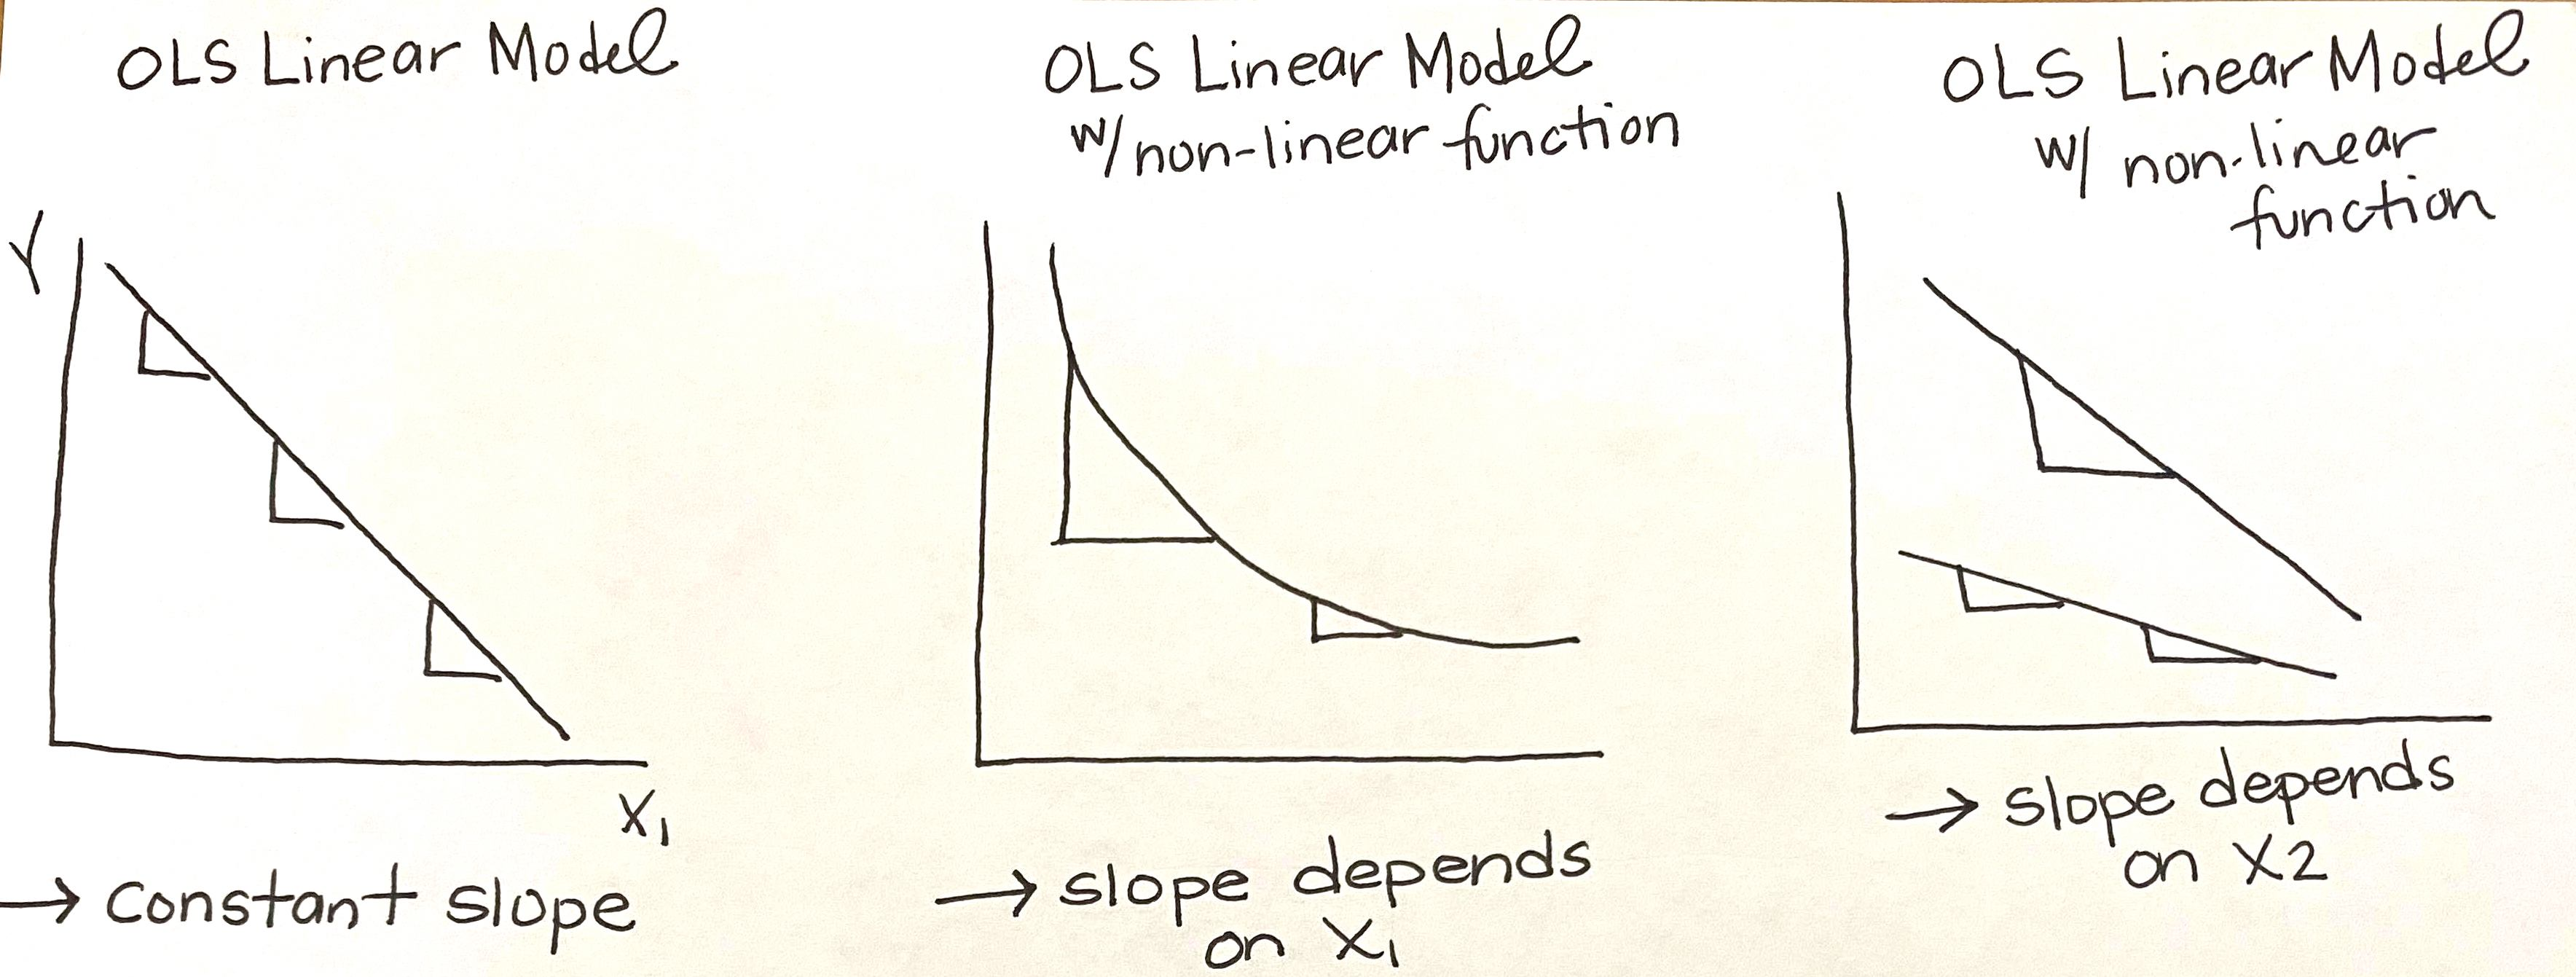
\includegraphics{slope.jpg}

\end{frame}

\hypertarget{introduction-to-interaction-effects}{%
\section{Introduction to Interaction
Effects}\label{introduction-to-interaction-effects}}

\begin{frame}{What are interaction effects?}
\protect\hypertarget{what-are-interaction-effects}{}

\begin{itemize}
\tightlist
\item
  Simple hypothesis

  \begin{itemize}
  \tightlist
  \item
    X has an effect on Y
  \item
    Ex: Participation in MAS (X) has an effect on graduation (Y)
  \end{itemize}
\item
  Interactions = Conditional Hypothesis

  \begin{itemize}
  \tightlist
  \item
    The effect of X on Y depends on a third variable
  \item
    Ex: the effect of MAS participation (X) on graduation (Y) differs by
    race (Z)
  \end{itemize}
\item
  What is an interaction effect? (i.e., ``moderators'')

  \begin{itemize}
  \tightlist
  \item
    An interaction effect is when the relationship between two variables
    (X and Y) depends on the value of a third variable Z
  \end{itemize}
\end{itemize}

\end{frame}

\begin{frame}{Interaction Effects}
\protect\hypertarget{interaction-effects}{}

\begin{itemize}
\tightlist
\item
  Interaction Effects are difficult!

  \begin{itemize}
  \tightlist
  \item
    It takes a while (and lots of practice!) to get comfortable thinking
    about and interpreting interaction effects
  \end{itemize}
\item
  I will provide an ``introduction'' to interaction effects!

  \begin{itemize}
  \tightlist
  \item
    We will continue to learn interaction effects in HED 613
  \item
    If you don't take HED 613, seek out more opportunities to learn
    interaction effects!
  \item
    Read empirical pieces that use/interpret interaction effects!
  \end{itemize}
\end{itemize}

\end{frame}

\begin{frame}{Three cases of interaction effects}
\protect\hypertarget{three-cases-of-interaction-effects}{}

\textbf{1. Interaction between a categorical and continous variable}
{[}today{]}

\begin{itemize}
\tightlist
\item
  Example: the effect of years of schooling (X) on earnings (Y) differs
  by gender (Z)
\end{itemize}

\textbf{2. Interaction between two categorical variables} {[}next
week{]}

\begin{itemize}
\tightlist
\item
  Example: the effect of highest degree attained (X) on earnings (Y)
  differs by gender (Z)
\end{itemize}

\textbf{3. Interaction between two continuous variables} {[}next week{]}

\begin{itemize}
\tightlist
\item
  Example: the effect of years of schooling (X) on earnings (Y) differs
  by age (Z)
\end{itemize}

\end{frame}

\hypertarget{interactions-between-a-categorical-and-continous-variable}{%
\section{Interactions between a categorical and continous
variable}\label{interactions-between-a-categorical-and-continous-variable}}

\begin{frame}{Interaction between a categorical and continous variable}
\protect\hypertarget{interaction-between-a-categorical-and-continous-variable}{}

\textbf{RQ: Does the effect of years of schooling (X) on earnings (Y)
differ by gender (Z)?}

\begin{itemize}
\tightlist
\item
  Continuous by Categorical Interaction

  \begin{itemize}
  \tightlist
  \item
    Y = earnings
  \item
    X = years of schooling
  \item
    Z (interaction variable) = gender (1=women, 0=men)
  \end{itemize}
\item
  Simple hypothesis

  \begin{itemize}
  \tightlist
  \item
    Years of schooling affects earnings
  \end{itemize}
\item
  Conditional hypothesis (interaction effect)

  \begin{itemize}
  \tightlist
  \item
    The effect of years of schooling (X) on earnings (Y) depends on
    gender
  \item
    In other words:

    \begin{itemize}
    \tightlist
    \item
      Is the effect of years of schooling on earnings lower for women
      than men?
    \end{itemize}
  \end{itemize}
\end{itemize}

\end{frame}

\begin{frame}{Simple Regression (no interaction effect)}
\protect\hypertarget{simple-regression-no-interaction-effect}{}

\begin{itemize}
\tightlist
\item
  Simple Regression

  \begin{itemize}
  \tightlist
  \item
    What is the effect of years of schooling on earnings?
  \item
    Population regression model:

    \begin{itemize}
    \tightlist
    \item
      \(Y_i = \beta_0 + \beta_1X_{1i} + u_i\)
    \item
      where Y= earnings, \(X_{1}\) = years of schooling
    \end{itemize}
  \end{itemize}
\item
  Run model in R
\item
  \(earnings = \beta_0 + \beta_1*schooling_{i} + u_i\)

  \begin{itemize}
  \tightlist
  \item
    \(\hat{earnings} = \hat{\beta_0} + \hat{\beta_1}*schooling_{i}\)
  \item
    \(\hat{earnings} = -5.37626 + 1.74515*schooling_{i}\)
  \end{itemize}
\item
  \(\hat{\beta_1}\) = 1.74515

  \begin{itemize}
  \tightlist
  \item
    On average, a one-unit (i.e., one year) increase in schooling is
    associated with a \$1745.15 (1.74515*1000) increase in earnings
  \item
    \(\hat{\beta_1}\) is significant at the 0.000 level
  \end{itemize}
\end{itemize}

\end{frame}

\begin{frame}{Multivariate Regression (no interaction effect)}
\protect\hypertarget{multivariate-regression-no-interaction-effect}{}

\begin{itemize}
\tightlist
\item
  Multivariate Regression

  \begin{itemize}
  \tightlist
  \item
    What is the effect of years of schooling on earnings controlling for
    gender?
  \item
    Population regression model:

    \begin{itemize}
    \tightlist
    \item
      \(Y_i = \beta_0 + \beta_1X_{1i} + \beta_2X_{2i} + u_i\)
    \item
      where Y= earnings, \(X_{1}\) = years of schooling, \(X_{2}\) = 0/1
      women
    \end{itemize}
  \end{itemize}
\item
  Run model in R
\item
  \(\hat{Y_i} = \hat{\beta_0} + \hat{\beta_1}X_{1i} + \hat{\beta_2}X_{2i}\)

  \begin{itemize}
  \tightlist
  \item
    \(\hat{Y_i} = -4.10405 + 1.78714*X_{1i} + -4.18848*X_{2i}\)
  \end{itemize}
\item
  \(\hat{\beta_1}\) = 1.78714

  \begin{itemize}
  \tightlist
  \item
    On average, a one-unit (i.e., one year) increase in schooling is
    associated with a \$1787.14 (1.78714*1000) increase in earnings,
    controlling for gender
  \item
    \(\hat{\beta_1}\) is significant at the 0.000 level
  \end{itemize}
\item
  \(\hat{\beta_2}\) = -4.18848

  \begin{itemize}
  \tightlist
  \item
    On average, identifying as a woman as opposed to a man, is
    associated with a \$4188.48 (4.18848*1000) decrease in earnings,
    controlling for years of schooling
  \item
    \(\hat{\beta_2}\) is significant at the 0.000 level
  \end{itemize}
\end{itemize}

\end{frame}

\begin{frame}{Simple and Multivariate Regression (no interaction
effects)}
\protect\hypertarget{simple-and-multivariate-regression-no-interaction-effects}{}

\begin{itemize}
\tightlist
\item
  Simple hypotheses on the multivariate model that controls for gender
  forces \textbf{the effect of years of schooling} to be the same for
  men and women

  \begin{itemize}
  \tightlist
  \item
    They have the same slope!
  \end{itemize}
\item
  But we want to investigate whether the effect of schooling differs for
  men and women!
\item
  Let's plot in R to see why we think men and women have different
  effects (i.e., different slopes!)

  \begin{itemize}
  \tightlist
  \item
    Seems like women get greater returns on college education, despite
    earning less.
  \item
    Lot of research seeks to answer why\ldots{}
  \end{itemize}
\item
  For continuous by categorical interactions, an alternative is to just
  run the regular OLS model (without interactions) for each group of Z!

  \begin{itemize}
  \tightlist
  \item
    This is pretty simple for binary variable, but more time consuming
    for 2+ categories
  \end{itemize}
\end{itemize}

\end{frame}

\begin{frame}{Seperate Models for each group of Z}
\protect\hypertarget{seperate-models-for-each-group-of-z}{}

\begin{itemize}
\tightlist
\item
  What is the effect of years of schooling on earnings for women?

  \begin{itemize}
  \tightlist
  \item
    Run model in R
  \item
    \(\hat{Y_i} = -9.4450 + 1.8950*X_{1i}\)
  \item
    \(\hat{\beta_0}\): predicted earnings when years of schooling is
    zero for women

    \begin{itemize}
    \tightlist
    \item
      Non-sensical but some substantive meaning relative to men model
    \end{itemize}
  \item
    \(\hat{\beta_1}\): On average, a one-unit (i.e., one year) increase
    in schooling is associated with a \$1895.00 (1.8950*1000) increase
    in earnings \emph{for women}
  \end{itemize}
\item
  What is the effect of years of schooling on earnings for men?

  \begin{itemize}
  \tightlist
  \item
    Run model in R
  \item
    \(\hat{Y_i} = -3.2368 + 1.6948*X_{1i}\)
  \item
    \(\hat{\beta_0}\): predicted earnings when years of schooling is
    zero for men

    \begin{itemize}
    \tightlist
    \item
      Men are predicted to have greater earnings than women when years
      of schooling is zero
    \end{itemize}
  \item
    \(\hat{\beta_1}\): On average, a one-unit (i.e., one year) increase
    in schooling is associated with a \$1694.80 (1.6948*1000) increase
    in earnings \emph{for men}
  \end{itemize}
\end{itemize}

\end{frame}

\begin{frame}{Seperate Models for each group of Z}
\protect\hypertarget{seperate-models-for-each-group-of-z-1}{}

\begin{itemize}
\tightlist
\item
  Plot matches results for seperate models

  \begin{itemize}
  \tightlist
  \item
    Our lines have different slopes

    \begin{itemize}
    \tightlist
    \item
      Women have slightly steeper line
    \end{itemize}
  \item
    Womens intercept is below mens
  \end{itemize}
\end{itemize}

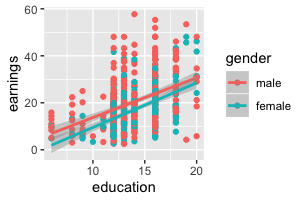
\includegraphics{Rplot01.png}

\end{frame}

\begin{frame}{Interaction Model for Continuous by Categorical Variables}
\protect\hypertarget{interaction-model-for-continuous-by-categorical-variables}{}

\begin{itemize}
\tightlist
\item
  Let's run an interaction effect between years of schooling and gender

  \begin{itemize}
  \tightlist
  \item
    This will allow the effect of years of schooling on earnings to
    differ by gender
  \end{itemize}
\item
  Population regression model

  \begin{itemize}
  \tightlist
  \item
    \(Y_i = \beta_0 + \beta_1X_{1i} + \beta_2Z_{i} + \beta_3(X_{1i}*Z_{i}) + u_i\)

    \begin{itemize}
    \tightlist
    \item
      where Y= earnings, \(X_{1}\) = years of schooling, \(Z_{i}\) = 0/1
      women
    \item
      \(X_{1i}*Z_{i}\) = interaction for years of schooling and gender
    \end{itemize}
  \end{itemize}
\end{itemize}

\medskip

\begin{itemize}
\tightlist
\item
  OLS Prediction line without estimates

  \begin{itemize}
  \tightlist
  \item
    \(\hat{Y_i} = \hat{\beta_0} + \hat{\beta_1}X_{1i} + \hat{\beta_2}Z_{i} + \hat{\beta_3}(X_{1i}*Z_{i})\)
  \end{itemize}
\end{itemize}

\medskip

\begin{itemize}
\tightlist
\item
  \textbf{\(\hat{\beta_0}\) = \(\hat{Y_i}\) when X1=0 and Z=0}

  \begin{itemize}
  \tightlist
  \item
    Predicted earnings for men (Z=0) with zero years of schooling (X1=0)
  \end{itemize}
\item
  \textbf{\(\hat{\beta_1}\) = change in \(\hat{Y_i}\) for a one-unit
  increase in X1, when Z=0}

  \begin{itemize}
  \tightlist
  \item
    change in earnings for a one-year increase in years of schooling for
    men (Z=0)
  \end{itemize}
\item
  \textbf{\(\hat{\beta_2}\) = change in \(\hat{Y_i}\) for a one-unit
  incease in Z, when X1=0}

  \begin{itemize}
  \tightlist
  \item
    change in earnings for women as opposed to men with zero years of
    schooling
  \end{itemize}
\item
  \textbf{\(\hat{\beta_3}\) = interaction term: how much the effect of
  X1 on \(\hat{Y_i}\) changes when Z increases by one unit}

  \begin{itemize}
  \tightlist
  \item
    change in the effect of years of schooling on earnings for a
    one-unit increase in Z
  \end{itemize}
\end{itemize}

\end{frame}

\begin{frame}[fragile]{Interaction Model for Continuous by Categorical
Variables}
\protect\hypertarget{interaction-model-for-continuous-by-categorical-variables-1}{}

\begin{itemize}
\tightlist
\item
  Let's run an interaction effect between years of schooling and gender

  \begin{itemize}
  \tightlist
  \item
    This will allow the effect of years of schooling on earnings to
    differ by gender
  \end{itemize}
\item
  We can create the interaction variable!

  \begin{itemize}
  \tightlist
  \item
    Generally: Multiply the X var by Z var
  \item
    in R: \texttt{df\$int\_xz\ \textless{}-\ df\$x*df\$z}
  \item
    creating variables may take a bit more ``R knowledge''
  \end{itemize}
\item
  Or just use R shortcut!
\item
  \texttt{lm(Y\ \textasciitilde{}\ X\ +\ Z\ +\ X:Z,\ data\ =\ df)}
\item
  \textbf{NOTE}: \emph{always} include X, Z, and X*Z
\end{itemize}

\medskip

\begin{itemize}
\tightlist
\item
  \(\hat{Y_i} = \hat{\beta_0} + \hat{\beta_1}X_{1i} + \hat{\beta_2}Z_{i} + \hat{\beta_3}(X_{1i}*Z_{i})\)
  \(\hat{Y_i} = -3.2368 + 1.6948*X_{1i} - 6.2082*Z_{i} + 0.2002*(X_{1i}*Z_{i})\)
\end{itemize}

\end{frame}

\begin{frame}{What do we want to know from interactions?}
\protect\hypertarget{what-do-we-want-to-know-from-interactions}{}

\begin{enumerate}
\item
  Is there an interaction effect?
\item
  What is the predicted value of Y for Z=0 and Z=1 at different values
  of X?
\item
  What is the effect of X on Y for different values of Z?
\end{enumerate}

\end{frame}

\begin{frame}{Is there an interaction effect?}
\protect\hypertarget{is-there-an-interaction-effect}{}

\begin{itemize}
\tightlist
\item
  Is the effect of years of schooling on earnings significantly
  different for women vs men?

  \begin{itemize}
  \tightlist
  \item
    \(Y_i = \beta_0 + \beta_1X_{1i} + \beta_2Z_{i} + \beta_3(X_{1i}*Z_{i}) + u_i\)
  \end{itemize}
\item
  Hypothesis test

  \begin{itemize}
  \tightlist
  \item
    \(H_0: \beta_3 =0\) vs \(H_0: \beta_3 \ne 0\)
  \item
    In other words, test whether the beta coefficient for the
    interaction term is significantly different from zero. If so, then
    there is an interaction!
  \end{itemize}
\item
  \(\hat{\beta_3}\) = 0.2002 , p-value of 0.494

  \begin{itemize}
  \tightlist
  \item
    We cannot reject \(H_0\) at \(\alpha\) of 0.05
  \end{itemize}
\item
  Magnitude

  \begin{itemize}
  \tightlist
  \item
    If \(\hat{\beta_3}\) is greater than zero (and statistically
    significant!) the effect of X on Y is larger when Z=1 than when Z=0
  \item
    If \(\hat{\beta_3}\) is less than zero (and statistically
    significant!) the effect of X on Y is smaller when Z=1 than when Z=0
  \end{itemize}
\end{itemize}

\end{frame}

\begin{frame}{What is the predicted value of Y for Z=0 and Z=1 at
different values of X}
\protect\hypertarget{what-is-the-predicted-value-of-y-for-z0-and-z1-at-different-values-of-x}{}

\begin{itemize}
\tightlist
\item
  What is the predicted earnings (Y) for men (Z=0) with 12 years of
  schooling?

  \begin{itemize}
  \tightlist
  \item
    \(\hat{Y_i} = \hat{\beta_0} + \hat{\beta_1}X_{1i} + \hat{\beta_2}Z_i + \hat{\beta_3}(X_{1i}*Z_i)\)
  \item
    Z=0 \& X=12:
    \(\hat{Y_i} = -3.2368 + (1.6948*12) - (6.2082*0) + (0.2002*(12*0))\)
  \item
    \(\hat{Y_i} = -3.2368 + (1.6948*12)\)
  \item
    \(\$17.1k = -3.2368 + (20.3376)\)
  \end{itemize}
\end{itemize}

\medskip

\begin{itemize}
\tightlist
\item
  What is the predicted earnings (Y) for women (Z=1) with 12 years of
  schooling?

  \begin{itemize}
  \tightlist
  \item
    \(\hat{Y_i} = \hat{\beta_0} + \hat{\beta_1}X_{1i} + \hat{\beta_2}Z_i + \hat{\beta_3}(X_{1i}*Z_i)\)
  \item
    Z=1 \& X=12:
    \(\hat{Y_i} = -3.2368 + (1.6948*12) - (6.2082*1) + (0.2002*(12*1))\)
  \item
    \(\hat{Y_i} = -3.2368 + (1.6948*12) - (6.2082*1) + (0.2002*12)\)
  \item
    \(\$13.3k = -3.2368 + (20.3376) - (6.2082) + (2.4024)\)
  \end{itemize}
\end{itemize}

\medskip

\begin{itemize}
\tightlist
\item
  Same result as when we ran model seperately by sample!

  \begin{itemize}
  \tightlist
  \item
    Men: \(\hat{Y_i}\) = -3.2368 + (1.6948*12) = 17.1008
  \item
    Women: \(\hat{Y_i}\) = -9.4450 + (1.8950*12) = 13.295
  \end{itemize}
\item
  But running seperately by sample does not test whether there is a
  statistically significant interaction!
\end{itemize}

\end{frame}

\begin{frame}{What is the effect of X on Y for different values of Z}
\protect\hypertarget{what-is-the-effect-of-x-on-y-for-different-values-of-z}{}

\begin{itemize}
\tightlist
\item
  \(\hat{Y_i} = \hat{\beta_0} + \hat{\beta_1}X_{1i} + \hat{\beta_2}Z_i + \hat{\beta_3}(X_{1i}*Z_i)\)

  \begin{itemize}
  \tightlist
  \item
    Remember that:
  \item
    \(\hat{\beta_1}\) = change in \(\hat{Y_i}\) for a one-unit increase
    in X1, when Z=0 -- \(\hat{\beta_1}\) = how much effect of X1 on Y
    changes when Z increases by one unit
  \end{itemize}
\end{itemize}

\medskip

\begin{itemize}
\tightlist
\item
  Predicted outcome if Z=0

  \begin{itemize}
  \tightlist
  \item
    \(\hat{Y_i} = \hat{\beta_0} + \hat{\beta_1}X_{1i} + \hat{\beta_2}*0 + \hat{\beta_3}(X_{1i}*0)\)
  \item
    \(\hat{Y_i} = \hat{\beta_0} + \hat{\beta_1}X_{1i}\)
  \item
    \textbf{\(\hat{\beta_1}\): Average effect of X on Y when Z=0}
  \end{itemize}
\end{itemize}

\medskip

\begin{itemize}
\tightlist
\item
  Predicted outcome if Z=1

  \begin{itemize}
  \tightlist
  \item
    \(\hat{Y_i} = \hat{\beta_0} + \hat{\beta_1}X_{1i} + \hat{\beta_2}*1 + \hat{\beta_3}(X_{1i}*1)\)
  \item
    \(\hat{Y_i} = \hat{\beta_0} + \hat{\beta_1}X_{1i} + \hat{\beta_2} + \hat{\beta_3}X_{1i}\)
  \item
    \(\hat{Y_i} = \hat{\beta_0} + \hat{\beta_2} + (\hat{\beta_1} + \hat{\beta_3})X_{1i}\)
  \item
    \textbf{\((\hat{\beta_1} + \hat{\beta_3})\): Average effect of X on
    Y when Z=1}
  \end{itemize}
\end{itemize}

\end{frame}

\begin{frame}{What is the effect of X on Y for different values of Z}
\protect\hypertarget{what-is-the-effect-of-x-on-y-for-different-values-of-z-1}{}

\begin{itemize}
\tightlist
\item
  \(\hat{Y_i} = \hat{\beta_0} + \hat{\beta_1}X_{1i} + \hat{\beta_2}*1 + \hat{\beta_3}(X_{1i}*1)\)
\item
  \(\hat{Y_i} = -3.2368 + 1.6948*X_{1i} - 6.2082*Z_i + 0.2002(X_{1i}*Z_i)\)

  \begin{itemize}
  \tightlist
  \item
    Remember that:
  \item
    \(\hat{\beta_1}\) = change in \(\hat{Y_i}\) for a one-unit increase
    in X1, when Z=0 -- \(\hat{\beta_1}\) = how much effect of X1 on Y
    changes when Z increases by one unit
  \end{itemize}
\end{itemize}

\medskip

\begin{itemize}
\tightlist
\item
  \textbf{\(\hat{\beta_1}\): Average effect of X on Y when Z=0}

  \begin{itemize}
  \tightlist
  \item
    \(\hat{\beta_1}\) = 1.6948
  \item
    On average, a one-year increase in years of schooling (X) is
    associated with \$1,694.80 (1.6948*1000) increase in earnings for
    men (Z=0)
  \end{itemize}
\end{itemize}

\medskip

\begin{itemize}
\tightlist
\item
  \textbf{\((\hat{\beta_1} + \hat{\beta_3})\): Average effect of X on Y
  when Z=1}

  \begin{itemize}
  \tightlist
  \item
    \(\hat{\beta_1}\) = 1.6948; \(\hat{\beta_3}\) = 0.2002
  \item
    1.6948 + 0.2002 = 1.895
  \item
    On average, a one-year increase in years of schooling (X) is
    associated with \$1,895.00 (1.895*1000) increase in earnings for
    women (Z=1)
  \end{itemize}
\end{itemize}

\medskip

\begin{itemize}
\tightlist
\item
  Same result as when we ran model seperately by sample!
\end{itemize}

\end{frame}

\hypertarget{klasik-blagg-pekor-2018}{%
\section{Klasik, Blagg, Pekor (2018)}\label{klasik-blagg-pekor-2018}}

\begin{frame}{Klasik, Blagg, Pekor (2018)}
\protect\hypertarget{klasik-blagg-pekor-2018-1}{}

\begin{itemize}
\tightlist
\item
  \textbf{RQs}: What is the relationship between living in a higher
  education desert and where a student applies to?

  \begin{itemize}
  \tightlist
  \item
    Education deserts: areas with very few higher education institutions
    or areas with where limited higher education instituions are 2-year
    colleges
  \item
    We know there are disparities in who lives in education deserts
  \item
    How what is ``the effect'' of living in an education desert on
    college application and enrollment decisions

    \begin{itemize}
    \tightlist
    \item
      They use ``related'' because it's not a program evaluation
      empirical strategy!
    \end{itemize}
  \end{itemize}
\item
  \textbf{Empirical Strategy Used}

  \begin{itemize}
  \tightlist
  \item
    Descriptive and relational; not program evaluation work!
  \end{itemize}
\item
  \textbf{Data: Educational Longitudinal Survey of 2002}

  \begin{itemize}
  \tightlist
  \item
    Dependent Variable(s): college application and enrollment behavior

    \begin{itemize}
    \tightlist
    \item
      Y1 = 0/1 applied to college outside their CZ
    \item
      Y2 = 0/1 enrolled in college outside their CZ
    \item
      Y3 = 0/1 applied to a matched college
    \item
      Y4 = 0/1 emrolled in a matched college
    \end{itemize}
  \item
    Independent variables of interest: variables related to education
    deserts

    \begin{itemize}
    \tightlist
    \item
      X1 = 0/1 lives in an access desert. (access deserts: students
      overall have few higher education institutions in close proximity
      to where they live)
    \item
      X1 = 0/1 lives in a match desert. (match deserts: students have
      few higher education institutions that \emph{match} their academic
      prepration in close proximity to where they live)
    \end{itemize}
  \end{itemize}
\item
  \textbf{Linear Probability Model}

  \begin{itemize}
  \tightlist
  \item
    \(Y_i = \beta_0 + \beta_1Desert_i + Xi\beta_2 + u_i\)
  \item
    Where X\_i is a vector of control variables:

    \begin{itemize}
    \tightlist
    \item
      race/ethnicity, family income, GPA, special education
      qualifications, AP work, single parent household, first-gen, etc.
    \end{itemize}
  \end{itemize}
\end{itemize}

\end{frame}

\begin{frame}{Klasik, Blagg, Pekor (2018)}
\protect\hypertarget{klasik-blagg-pekor-2018-2}{}

\begin{itemize}
\tightlist
\item
  Table 3: Relationship between living in access desert and applying to
  college outside of home commuting zone

  \begin{itemize}
  \tightlist
  \item
    Dependent variable is applied to college outside of CZ (Y1)
  \item
    Independent variable of interest is lives in an Access Desert
  \item
    Columns are different models; progression from intercept model to
    adding controls
  \item
    Rows indicate independent variable of interest and controls
  \item
    Good example of a program evaluation regression table!

    \begin{itemize}
    \tightlist
    \item
      We don't care about the coefficients on controls
    \item
      We only care about interpreting \(\hat{\beta_1}\)
    \end{itemize}
  \end{itemize}
\end{itemize}

\medskip

\begin{itemize}
\tightlist
\item
  Table 4: Dependent variable is enrolling in college outside of CZ (Y2)
  and independent variable is lives in an access desert (X1)
\item
  Table 5: Dependent variable is applying in a match college (Y3) and
  independent variable is lives in a match desert (X1)
\item
  Table 5: Dependent variable is enrolling in a match college (Y3) and
  independent variable is lives in a match desert (X1)
\end{itemize}

\end{frame}

\begin{frame}{Klasik, Blagg, Pekor (2018)}
\protect\hypertarget{klasik-blagg-pekor-2018-3}{}

\begin{itemize}
\tightlist
\item
  From lecture 13, Linear Probability Model

  \begin{itemize}
  \tightlist
  \item
    When X = categorical
  \item
    \(\hat{\beta_1}\): On average, being in the ``non-reference group''
    as opposed to the ``reference group'' is associated with a
    100*\(\hat{\beta_1}\) percentage point change in the probability of
    Y=1
  \end{itemize}
\end{itemize}

\textbf{Klasik, Blagg, Pekor (2018)}

\begin{itemize}
\item
  Table 3: Column 6 (all controls included)

  \begin{itemize}
  \tightlist
  \item
    \(\hat{\beta_1}\) = 0.189**
  \item
    On average, living in an access desert as opposed to not living in
    an access desert is associated with a 18.9 (100*0.189) percentage
    point increase in the probability of applying to a college outside
    their commuting zones, holding all covariates constant
  \item
    From authors pg 11: ``The students who live in an access desert are
    19 percentage points more likely to apply out of their commuting
    zone, relative to those who do not live in access deserts, even
    after controlling for the student's race, family background,
    coursework, and SAT score''
  \end{itemize}
\item
  Table 4: Column 6 (all controls included)

  \begin{itemize}
  \tightlist
  \item
    \(\hat{\beta_1}\) = 0.255**
  \item
    On average, living in an access desert as opposed to not living in
    an access desert is associated with a 25.5 (100*0.255) percentage
    point increase in the probability of enrolling in a college outside
    their commuting zones, holding all covariates constant
  \item
    From authors pg 11: ``Similarly, as shown in Table 4, the students
    in an access desert are roughly 26 percentage points more likely to
    enroll in a college outside of their commuting zone, even after
    controlling for a full set of demographic characteristics''
  \end{itemize}
\end{itemize}

\end{frame}

\end{document}
